\section{Survey Methodology}\label{sec:method}

\subsection{Research Objectives}

This survey will introduce the art of prompting from a big picture of artificial general intelligence (AGI). We first present three fundamental problems towards AGI in Table \ref{tab:rqs}. Recently, prompt learning has been demonstrated as a promising solution to these problems in many linear data such as text \cite{brown2020language, gao2021making}, images \cite{
% radford2021learning, 
wang2023chatvideo}, etc. However, whether the prompt technique can still solve these problems in the graph area, is not clearly discussed. Through this survey, we wish to figure out how the graph prompt potentially helps graph models to be more general across various tasks and domains, and how it generalizes the foundation models to interact with other modalities (e.g. text, image, etc). Beyond the above common problems of AGI in NLP, CV, and graph areas, graph prompting is usually very different from its counterparts in NLP and CV areas, leading to many detailed questions as shown in Table \ref{tab:rqs}. 

% the following content can be removed 
% By answering these detailed questions, we wish to achieve the following objectives:

% \begin{itemize}
%     \item Unifying Diverse Approaches for Understanding Existing Work. A unified framework to consolidate varied approaches in graph prompting is needed so that we can facilitate a comprehensive understanding of existing methodologies.
%     \item Diving into the Purpose of Prompts in the Graph Learning. To achieve this goal, we need to explore the inherent nature and strategic roles of prompts in graphs, which are mostly not as straightforward as the ones in the language area.
%     \item Designing Effective Graph Prompts. By summarizing the most representative works in graph prompts, we wish to find a fundamental creation in the design of graph prompts, focusing on creating efficient, versatile, and context-sensitive prompts that cater to specific requirements of graph-based tasks. 
%     % \item Assessing the Effectiveness of Graph Prompts. Currently, there are no widely accepted criteria for evaluating the effectiveness and efficiency of graph prompts, including their adaptability and scalability in different application scenarios. Proposing a comprehensive evaluation framework is a pressing need to further accelerate this research area.
%     \item  Implementing Graph Prompts in Real-World Scenarios. We need to provide a general programming tool to facilitate the practical implications of graph prompts in real-world settings, assessing their implementation challenges, and highlighting successful case studies. 
%     \item Identifying Challenges, Limitations and the Future of Graph Prompting. Currently, graph prompt research is very primitive and nascent, leaving many tough problems to be solved. By summarizing current challenges and future directions, we wish to push forward this research area to achieve more impact on related applications.
% \end{itemize}




\tikzstyle{leaf}=[draw=hiddendraw,
    rounded corners, minimum height=1em,
    fill=mygreen!40,text opacity=1, 
    fill opacity=.5,  text=black,align=left,font=\scriptsize,
    inner xsep=3pt,
    inner ysep=1pt,
    ]
\tikzstyle{middle}=[draw=hiddendraw,
    rounded corners, minimum height=1em,
    fill=output-white!40,text opacity=1, 
    fill opacity=.5,  text=black,align=center,font=\scriptsize,
    inner xsep=7pt,
    inner ysep=1pt,
    ]
\begin{figure*}[ht]
\centering
\begin{forest}
  for tree={
  forked edges,
  grow=east,
  reversed=true,
  anchor=base west,
  parent anchor=east,
  child anchor=west,
  base=middle,
  font=\scriptsize,
  rectangle,
  line width=0.7pt,
  draw=output-black,
  rounded corners,align=left,
  minimum width=2em, s sep=6pt, l sep=8pt,
  },
  where level=1{text width=0.2\linewidth}{},
  where level=2{text width=0.2\linewidth,font=\scriptsize}{},
  where level=3{font=\scriptsize}{},
  where level=4{font=\scriptsize}{},
  where level=5{font=\scriptsize}{},
  [Taxonomy, middle,rotate=90,anchor=north,edge=output-black
      [Pre-training Strategies for \\Graph Prompt (\secref{sec:pretrain_method}),middle,anchor=west,edge=output-black, text width=0.18\linewidth
        [{Node-level Strategies\\(\secref{subsec:node_pre})}, middle, text width=0.16\linewidth, edge=output-black
             [\citet{cheng2023wiener, zhu2021graph, jin2021multiscale, peng2020graph}\\\citet{hamilton2017inductive,hou2022graphmae,wang2021selfsuperviseda,wang2017mgae,park2019symmetric}\\\citet{hou2023graphmae2,wang2021selfsuperviseda,jiang2021pretraining}, leaf, text width=0.46\linewidth, edge=output-black] ]
        [{Edge-level Strategies\\(\secref{subsec:edge_pre})}, middle, text width=0.16\linewidth, edge=output-black
             [\citet{jin2021node, long2022pretraining,tan2023s2gae, li2023what,pan2018adversarially}\\\citet{ hasanzadeh2019semiimplicit, kim2021how}, leaf, text width=0.46\linewidth, edge=output-black] ]
        [{Graph-level Strategies\\(\secref{subsec:graph_pre})}, middle, text width=0.16\linewidth, edge=output-black
             [\citet{xie2022selfsupervised, rong2020selfsupervised,velickovic2019deep, sun2020infograph}\\\citet{sun2021mocl, subramonian2021motifdriven,you2020graph,suresh2021adversarial}\\\citet{ thakoor2021bootstrapped,qiu2020gcc}, leaf, text width=0.46\linewidth, edge=output-black]]
        [{Multi-task Pre-training\\(\secref{subsec:multi_pre})}, middle, text width=0.16\linewidth, edge=output-black
             [\citet{hu2020strategies, hu2020gptgnn, zhang2020graphbert,fang2022geometryenhanced}, leaf, text width=0.46\linewidth, edge=output-black] ]]
    [{Prompt Design for \\Graph Tasks (\secref{sec:ptask})}, middle,anchor=west,edge=output-black, text width=0.18\linewidth
        [{Prompt Token, Structure, and \\Inserting Pattern (\secref{subsec:pdesign})}, middle, text width=0.18\linewidth, edge=output-black
            [Prompt as Tokens, middle, text width=0.1\linewidth, edge=output-black [\citet{zhu2023graphcontrol,fang2022prompt,fang2023universal}\\\citet{gong2023prompt,tan2023virtual,liu2023graphprompt}\\\citet{zhu2023sglpt,ma2023hetgpt,sun2022gppt}\\\citet{chen2023ultradp,shirkavand2023deep}, leaf, text width=0.3\linewidth, edge=output-black]]
            [Prompt as Graphs, middle, text width=0.1\linewidth, edge=output-black
                [\citet{sun2023all,huang2023prodigy,ge2023enhancing}, leaf, text width=0.3\linewidth, edge=output-black] ] ]
        [Aligning Tasks by Answering \\Function (\secref{subsec:align}), middle, text width=0.18\linewidth, edge=output-black
             [Handling Different Level Tasks, middle, text width=0.18\linewidth, edge=output-black
             [\citet{sun2023all,huang2023prodigy}\\\citet{liu2023graphprompt,gong2023prompt}, leaf, text width=0.22\linewidth, edge=output-black] ]
              [Learnable Answering Function, middle, text width=0.18\linewidth, edge=output-black
                [\citet{sun2023all,fang2022prompt}\\\citet{fang2023universal,tan2023virtual}, leaf, text width=0.22\linewidth, edge=output-black]]
              [Hand-crafted Answering Function, middle, text width=0.2\linewidth, edge=output-black [\citet{sun2023all,sun2022gppt}\\\citet{ma2023hetgpt,ge2023enhancing}\\\citet{huang2023prodigy,liu2023graphprompt}, leaf, text width=0.2\linewidth, edge=output-black ]]]
        [{Prompt Tuning (\secref{subsec:pt})}, middle, text width=0.18\linewidth, edge=output-black
             [Meta-Learning Technique, middle, text width=0.2\linewidth, edge=output-black
                [\citet{sun2023all}, leaf, text width=0.2\linewidth, edge=output-black ] ]
             [Task-specific Tuning, middle, text width=0.2\linewidth, edge=output-black
                [\citet{fang2022prompt}, leaf, text width=0.2\linewidth, edge=output-black] ]
             [Tuning in Line with Pretext, middle, text width=0.2\linewidth, edge=output-black [\citet{liu2023graphprompt,sun2022gppt}\\\citet{tan2023virtual,ma2023hetgpt}\\\citet{ge2023enhancing,gong2023prompt}\\\citet{chen2023ultradp}, leaf, text width=0.2\linewidth, edge=output-black] ] ]
        [{Connection, Pros, and Cons\\(\secref{subsec:pdiscussion})}, middle, text width=0.18\linewidth, edge=output-black [\citet{fang2022prompt,fang2023universal,sun2023all,ma2023hetgpt,liu2023graphprompt}\\\citet{sun2022gppt,huang2023prodigy,chen2023ultradp,tan2023virtual}, leaf, text width=0.44\linewidth, edge=output-black] ] ]
    [Multi-Modal Prompting \\with Graphs (\secref{subsec:multi_modal}),middle, anchor=west, edge=output-black, text width=0.18\linewidth
         [Prompt in Text-Attributed Graphs, middle, text width=0.2\linewidth, edge=output-black
            [\citet{wen2023augmenting,wen2023prompt,zhao2023gimlet,li2023promptbased}, leaf, text width=0.42\linewidth, edge=output-black] ]
         [Large Language Models in Graph \\Data Processing, middle, text width=0.2\linewidth, edge=output-black
           [\citet{chen2023exploring,fatemi2023talk,jin2023patton,wang2023knowledge}, leaf, text width=0.42\linewidth, edge=output-black ] ]
         [Multi-modal Fusion with Graph \\and Prompting, middle, text width=0.2\linewidth, edge=output-black
           [\citet{edwards2023synergpt,li2023graphadapter,liu2023gitmol}, leaf, text width=0.42\linewidth, edge=output-black ] ]  ]
    [Graph Domain Adaptation\\ with Prompting (\secref{subsec:pdomain}),middle, anchor=west, edge=output-black, text width=0.18\linewidth
         [Semantic Alignment, middle, text width=0.2\linewidth, edge=output-black [\citet{sun2023all,zhu2023graphcontrol,zhang2023structure,yi2023contrastive}\\\citet{liu2023one}, leaf, text width=0.42\linewidth, edge=output-black ]
        ]
        [Structural Alignment, middle, text width=0.2\linewidth, edge=output-black
    [\citet{shirkavand2023deep,cao2023when,zhao2023graphglow}\\\citet{guo2023datacentric}, leaf, text width=0.42\linewidth, edge=output-black ] ] ]
]
\end{forest} 
\caption{Taxonomy of this Survey with Representative Works.}
\label{fig:Taxonomy}
\end{figure*}




\subsection{Taxonomy}

The taxonomy of this survey is presented in \figref{fig:Taxonomy}, which is intricately designed to categorize graph prompts based on their specific applications and functionalities, providing a structured approach to understanding their role in AGI. 



\textbf{(1) Pre-training Strategies for Graph Prompt.}

Since prompting techniques mostly seek to reformulate downstream tasks to the pre-training tasks, they are highly customized for detailed pre-training approaches, thus we briefly discuss the representative pre-training work in the graph area before we formally introduce graph prompt content. We split existing pre-training approaches into node-level, edge-level, graph-level, and multi-task pre-training strategies. Next, we present how different prompting ideas reformulate various downstream tasks to the corresponding pre-training tasks in the graph area. By revisiting existing pre-training literature, we will be more clear about the role of graph prompts in the whole "pre-training and prompting" framework.



\textbf{(2) Prompting Methods in Graph Areas.} 

Aiming at the three foundation problems mentioned in the research objectives (P1-P3 in \tabref{tab:rqs}), we analyze graph prompting from three aspects: \romannumeral1. prompt design for graph tasks (\secref{sec:ptask}); \romannumeral2. multi-modal prompting with graphs (\secref{subsec:pmodal}); and \romannumeral3. graph domain adaptation with prompting techniques (\secref{subsec:pdomain}). Within each aspect, we present a detailed discussion related to the five specific problems in the graph prompt area (Q1-Q5 in \tabref{tab:rqs}).

\textit{\romannumeral1. Prompt Design for Graph Tasks.} In this section, we propose a unified framework to analyze existing works on graph prompt design. Our framework treats existing graph prompts with three key components: \textit{prompt tokens}, which preserve prompt content as vectors; \textit{token structures}, which indicate how multiple tokens are organized; and \textit{inserting patterns}, which define how to combine graph prompt with the original graphs. Beyond that, we also carefully analyze how these works design the prompt answering function, which means how they get results for the downstream tasks from their  prompts. We also summarize three representative methods to learn appropriate prompts, including meta-learning techniques, task-specific tuning, and tuning in line with pretext. In the end, we further discuss these works in \secref{subsec:pdiscussion} to see their intrinsic connections with pros and cons.


\textit{\romannumeral2. Multi-modal Prompting with Graphs.} In this section, we briefly present how graph prompts work in a text-attributed graph, which can be seen as the fusion of text and graph modalities. With the progress of large language models (LLMs), the fusion of text and graph data has become easier and has aroused a lot of work on this topic. Since the topic of integrating LLMs with graphs has been well summarized in \cite{li2023survey}, we won't present too much in this survey. Instead, we only briefly discuss some representative works in this area that focus on the prompt area. 



\begin{table}[!t]
\centering
\caption{Research Objectives}
\label{tab:rqs}
% \resizebox{0.48\textwidth}{!}{%
\begin{tabular}{@{}l|l@{}}
\toprule
\multirow{3}{*}{\makecell[c]{Foundamental \\Problems\\ towards AGI}}  
        & \makecell[l]{P1: How to Make the Model General for Different\\ Modalities? (\secref{subsec:multi_modal}) } \\\cmidrule(l){2-2} 
        & \makecell[l]{P2: How to Make the Model General for Different \\Domains? (\secref{subsec:pdomain})} \\\cmidrule(l){2-2} 
        & \makecell[l]{P3: How to Make the Model General for Different \\Tasks?  (\secref{sec:ptask}) }  \\ \midrule
\multirow{5}{*}{\makecell[c]{Detailed \\Questions of\\ Graph Prompt}} 
        & \makecell[l]{Q1: How to Understand Existing Work with a \\Unified Framework? (\secref{subsec:pdesign})} \\\cmidrule(l){2-2} 
        & \makecell[l]{Q2: What's the Nature of Graph Prompt? \\(\secref{subsec:why_prompt}, \secref{subsec:pdiscussion})}   \\\cmidrule(l){2-2} 
        & \makecell[l]{Q3: How to Design Graph Prompts? (\secref{sec:ptask}) } \\\cmidrule(l){2-2} 
        % & \makecell[l]{How to Evaluate the Quality \\of Graph Prompts?     }    \\\cmidrule(l){2-2} 
        & \makecell[l]{Q4: How to Deploy Graph Prompts in Real-world \\Applications?  (\secref{sec:app}, \secref{sec:prog})}  \\\cmidrule(l){2-2} 
        & \makecell[l]{Q5: What Are the Current Challenges and Future \\Directions? (\secref{sec:challenges}) }   \\ \bottomrule
\end{tabular}%
% }
\end{table}



\textit{\romannumeral3. Graph Domain Adaptation through Prompting Techniques.} In this section, we introduce related work from two branches. The first branch presents works solving semantic alignment across different graph  domains, and the second branch presents structural alignment. 

\subsection{Literature Overview}
In this survey, we carefully studied more than 100 high-quality papers published within the past 5 years from reputable conferences and journals including but not limited to NeurIPS, SIGKDD, The Web Conference, ICLR, CIKM, ICML, IJCAI, EMNLP, SIGIR, ACL, AAAI, WSDM, TKDE, etc. Most of these venues are ranked as CCF A\footnote{\url{https://www.ccf.org.cn/Academic_Evaluation/By_category}} or CORA A*\footnote{\url{https://www.core.edu.au/conference-portal}}. Besides these works, we also introduce several latest works in arXiv so that our survey can catch up with the frontier and latest progress in this area. A more detailed pie chart (Figure \ref{fig:venue_dis}) presents the distribution of collected papers over these venues. Furthermore, we conducted an analysis of the topics covered by these references. In Figure \ref{fig:top10keys}, we present the top 15 keywords that appeared in the titles of these papers. Notably, these keywords align closely with the focus of our survey, which is centered around graph domains and prompt learning. 


\begin{figure*}[!t]
\centering
\subfloat[Venue distribution of collected papers.]{
\label{fig:venue_dis}
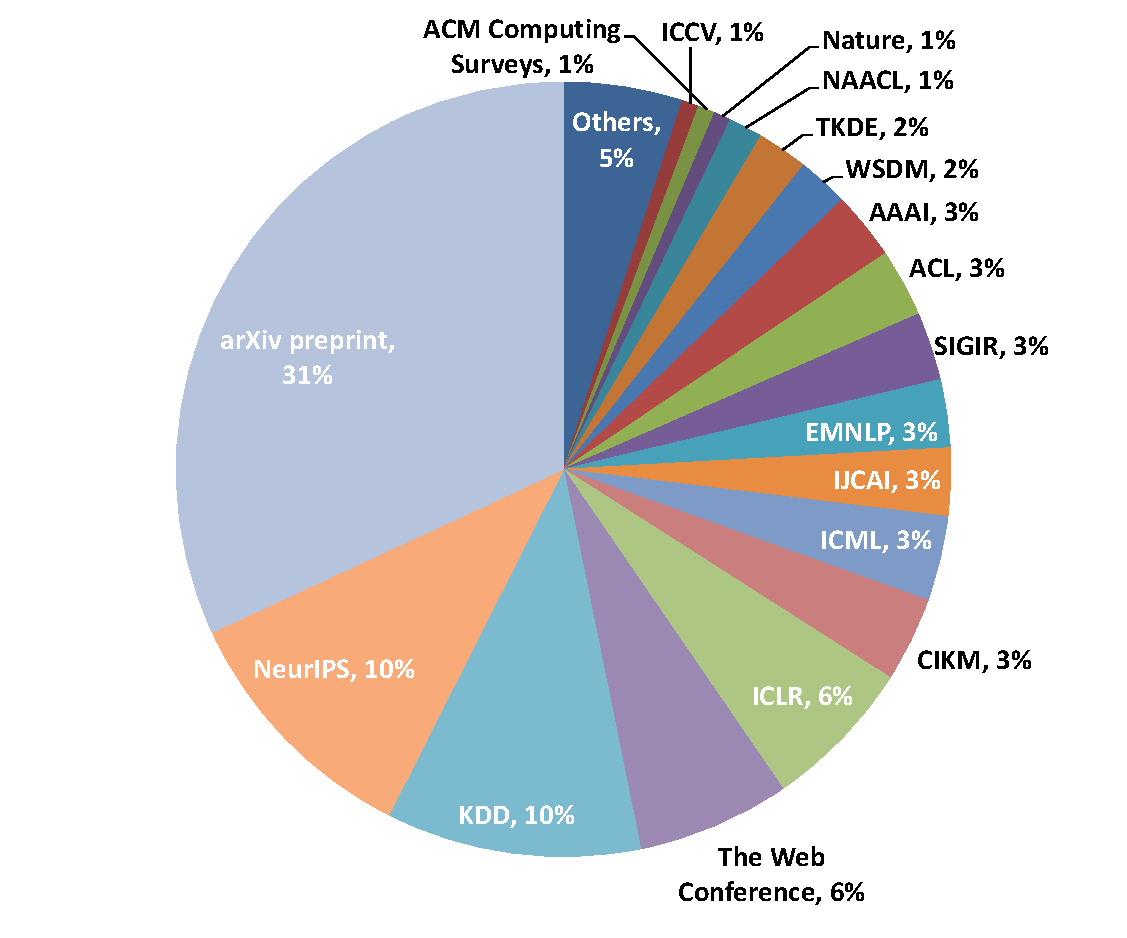
\includegraphics[width=0.4\textwidth]{pic/reference_venue.pdf}%
} 
\subfloat[Top 15 Keywords appeared in titles of collected papers]{
\label{fig:top10keys}
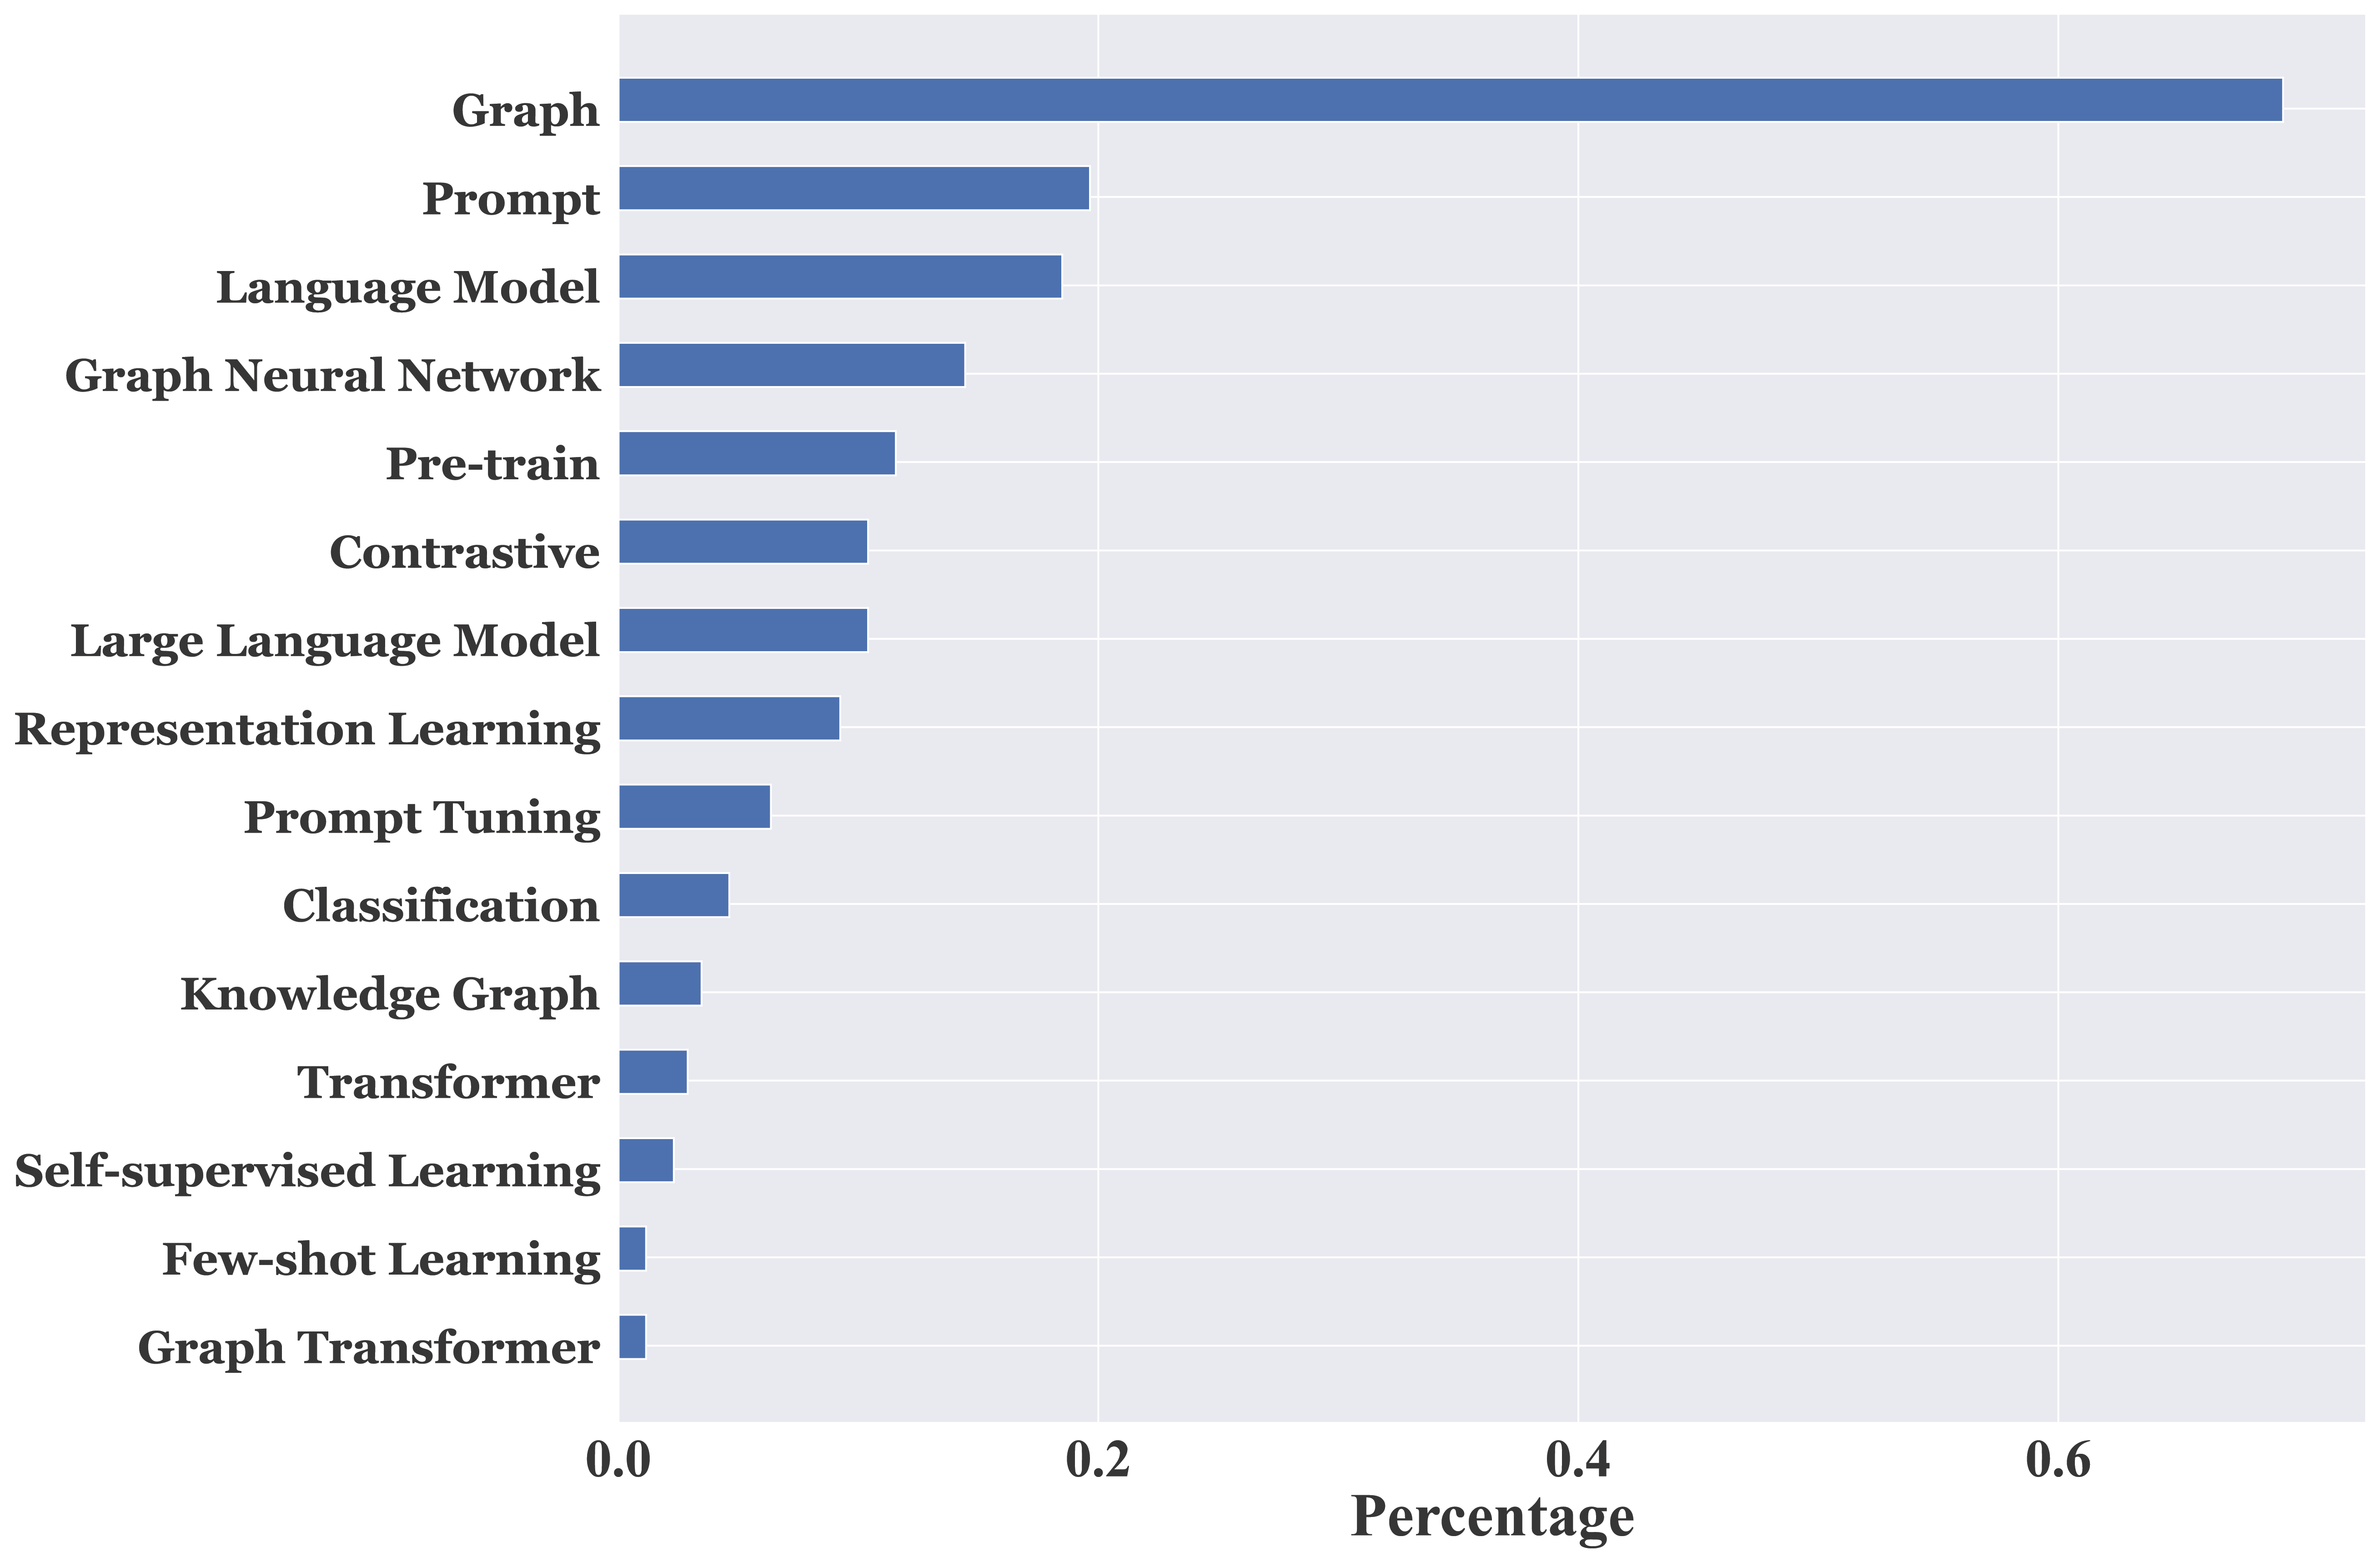
\includegraphics[width=0.5\textwidth]{pic/top_keywords_bar.png}%
}
\caption{Statistics of the collected papers}\vspace{-3ex}
\label{fig:credit_case}
\end{figure*}




\noindent \textbf{Connection to Existing Work: }

Our survey stands out from existing surveys in several notable ways. For example, \citet{liu2023graph} primarily focuses on graph foundation models (GFMs). Their survey does not specifically target graph prompts, and only a few papers in this area are briefly discussed. \citet{li2023survey} systematically analyze recent works that integrate graphs and LLMs, which is a detailed analysis of a small portion (Section \ref{subsec:multi_modal}) in our survey. We go beyond their scope by exploring various aspects of graph prompts in a more extensive manner. Meanwhile, surveys \cite{xie2023selfsupervised, yu2023selfsupervised} focus primarily on the pre-training stages, without involving the crucial aspect of graph prompt learning. While a prior survey on graph prompt learning by \citet{wu2023survey} exists, our survey surpasses it in several key aspects. Firstly, we provide \textbf{a more comprehensive analysis of related works}. Their survey was published in May 2023 when there were only a few graph prompt works available \cite{sun2022gppt, zhu2023sglpt, fang2022prompt}. In contrast, our survey encompasses a broader scope, including all relevant works in the field. Secondly, we offer \textbf{a systematic analysis of existing works} within a uniform framework, facilitating comprehension and comparison between different approaches. Thirdly, our survey provides deep insights into \textbf{the relationship between graph pre-training and prompts}, shedding light on the interplay between these critical elements. Lastly, we not only present empirical insights but also include \textbf{engineering works} aimed at deploying graph prompts in real-world applications, ensuring the practical applicability of our survey.